\documentclass[11pt,a4paper]{article}

\usepackage[utf8]{inputenc}
\usepackage[T1]{fontenc}
\usepackage[french]{babel}
\usepackage{geometry}
\usepackage{graphicx}
\usepackage{booktabs}
\usepackage{array}
\usepackage{float}
\usepackage{hyperref}

\geometry{margin=2.5cm}
\setlength{\parskip}{0.45em}
\setlength{\parindent}{0pt}

\title{Resultats de regression lineaire par periode et de split aleatoire\newline Feu en foret boreale}
\author{Projet Foret Boreale}
\date{\today}

\begin{document}
\maketitle

\section{Objectif}
Ce rapport resume deux analyses presentes dans le notebook \texttt{exploration\_variables\_modeles\_feu.BACKUP.ipynb}:
\begin{itemize}
\item une regression lineaire separee par periodes temporelles;
\item un benchmark avec split aleatoire et plusieurs modeles de base.
\end{itemize}

La variable cible est la colonne \texttt{Mean} des proxys feu, et la lecture doit se faire avec prudence: le split aleatoire a tendance a surestimer les performances lorsqu'il existe une forte autocorrelation temporelle.

\section{Regression lineaire par periode}

\subsection{Parametrage}
Le notebook applique une regression lineaire simple sur des fenetres de longueur variable. Les parametres utilises sont:
\begin{itemize}
\item tailles de periode testees: 100, 200, 300, 500, 1000, 1500 et 2000 ans;
\item proportion de test interne a chaque periode: 20\%;
\item nombre minimum d'observations par periode: 30;
\item metriques reportees: MAE, RMSE et $R^2$.
\end{itemize}

\subsection{Lecture des figures}
La premiere figure rappelle la distribution de la cible. Elle montre un signal bimodal ou du moins fortement asymetrique, avec un noyau principal autour de 0.64--0.66 et un second regime plus eleve vers 0.75--0.80.

\begin{figure}[H]
\centering
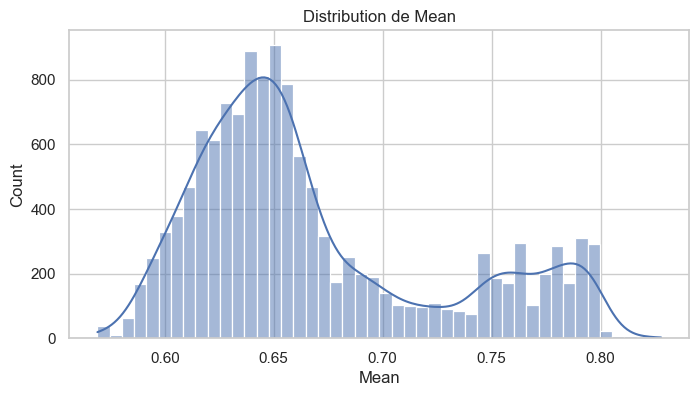
\includegraphics[width=0.88\textwidth]{figures_notebook_outputs/cell_009_output_06_01.png}
\caption{Distribution de la colonne \texttt{Mean} utilisee comme cible.}
\label{fig:mean_distribution}
\end{figure}

La figure suivante resume les scores par taille de periode. Le comportement est clair: les petites fenetres donnent des erreurs plus faibles, tandis que les fenetres longues degradent la qualite du fit et font chuter $R^2$.

\begin{figure}[H]
\centering
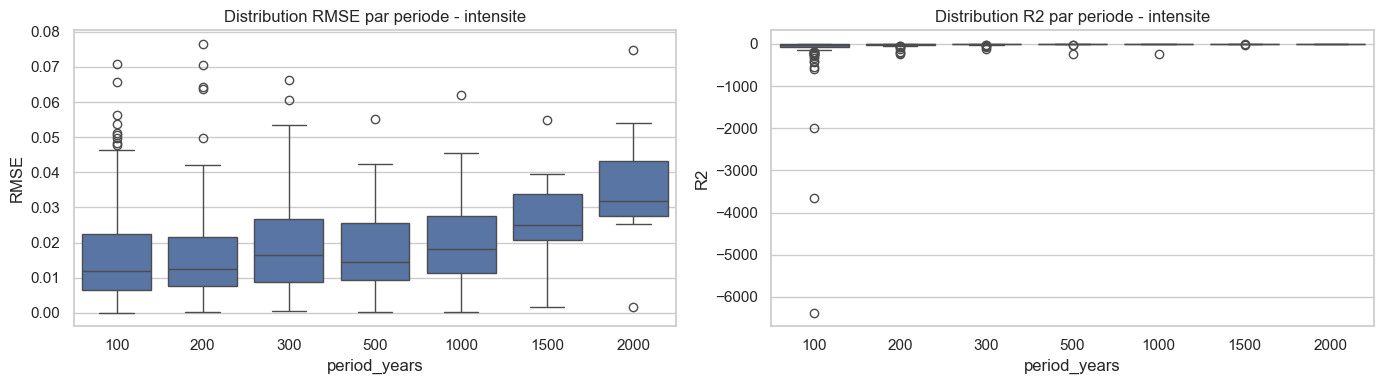
\includegraphics[width=0.95\textwidth]{figures_notebook_outputs/cell_009_output_11_02.png}
\caption{Distribution de la RMSE et du $R^2$ par taille de periode.}
\label{fig:period_metrics}
\end{figure}

Les graphiques de prediction montrent la comparaison entre observations et droite de regression pour plusieurs tailles de fenetres. On observe un accord relativement bon pour 100--500 ans, puis un lissage plus grossier lorsque la periode augmente.

\begin{figure}[H]
\centering
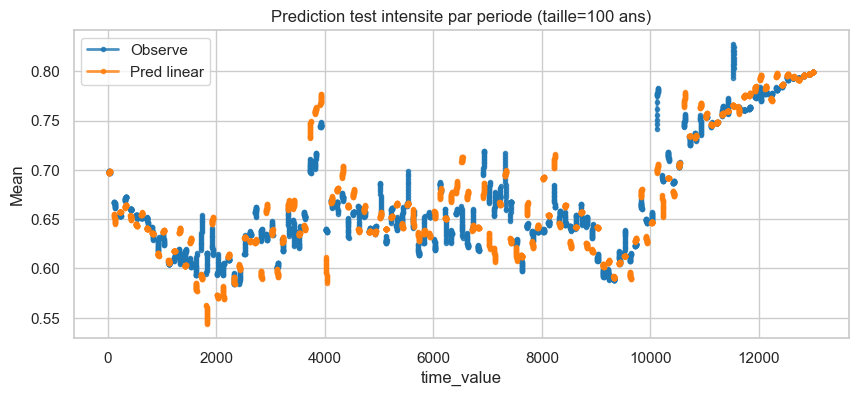
\includegraphics[width=0.92\textwidth]{figures_notebook_outputs/cell_009_output_12_03.png}
\caption{Prediction test pour une periode de 100 ans.}
\end{figure}

\begin{figure}[H]
\centering
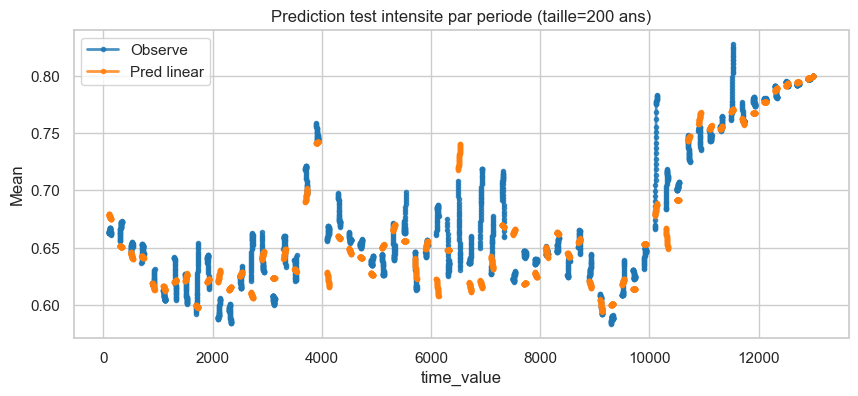
\includegraphics[width=0.92\textwidth]{figures_notebook_outputs/cell_009_output_13_04.png}
\caption{Prediction test pour une periode de 200 ans.}
\end{figure}

\begin{figure}[H]
\centering
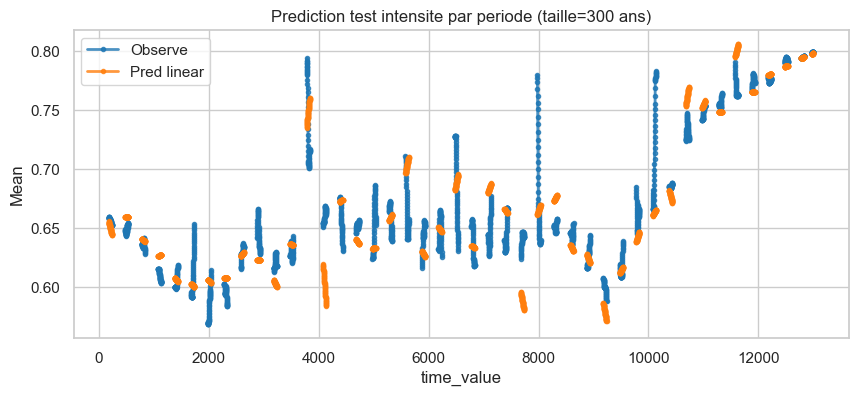
\includegraphics[width=0.92\textwidth]{figures_notebook_outputs/cell_009_output_14_05.png}
\caption{Prediction test pour une periode de 300 ans.}
\end{figure}

\begin{figure}[H]
\centering
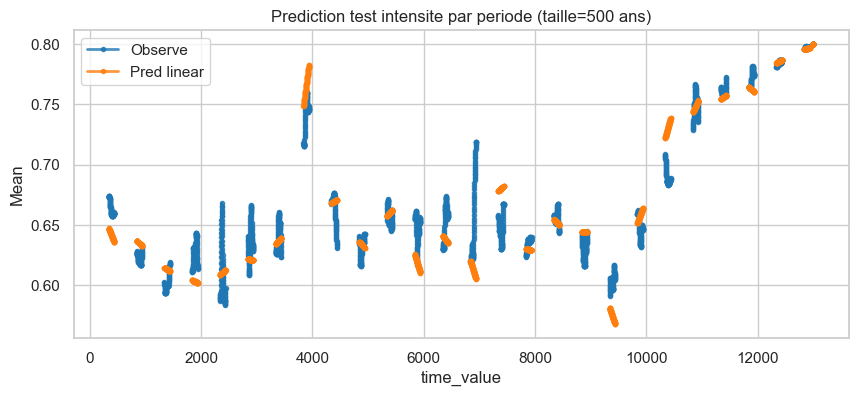
\includegraphics[width=0.92\textwidth]{figures_notebook_outputs/cell_009_output_15_06.png}
\caption{Prediction test pour une periode de 500 ans.}
\end{figure}

\begin{figure}[H]
\centering
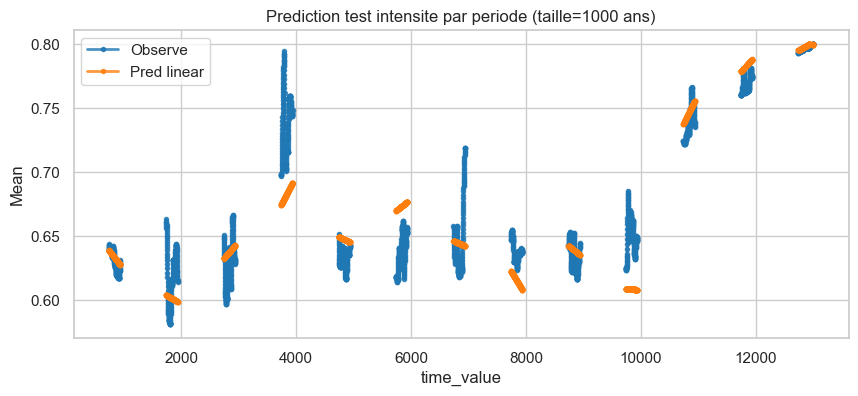
\includegraphics[width=0.92\textwidth]{figures_notebook_outputs/cell_009_output_16_07.png}
\caption{Prediction test pour une periode de 1000 ans.}
\end{figure}

\begin{figure}[H]
\centering
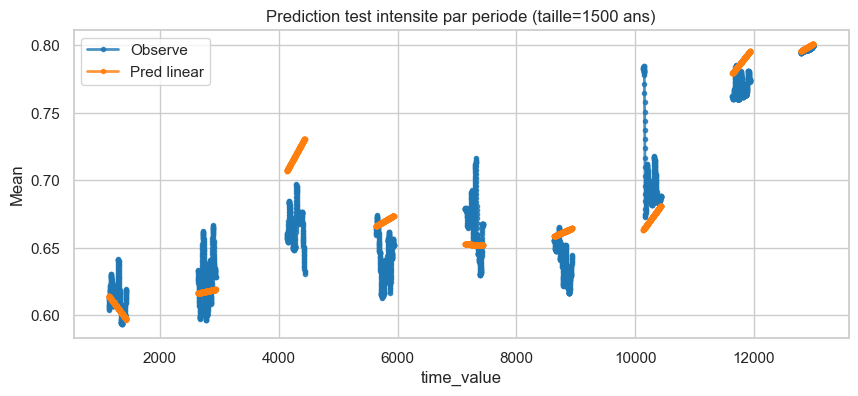
\includegraphics[width=0.92\textwidth]{figures_notebook_outputs/cell_009_output_17_08.png}
\caption{Prediction test pour une periode de 1500 ans.}
\end{figure}

\begin{figure}[H]
\centering
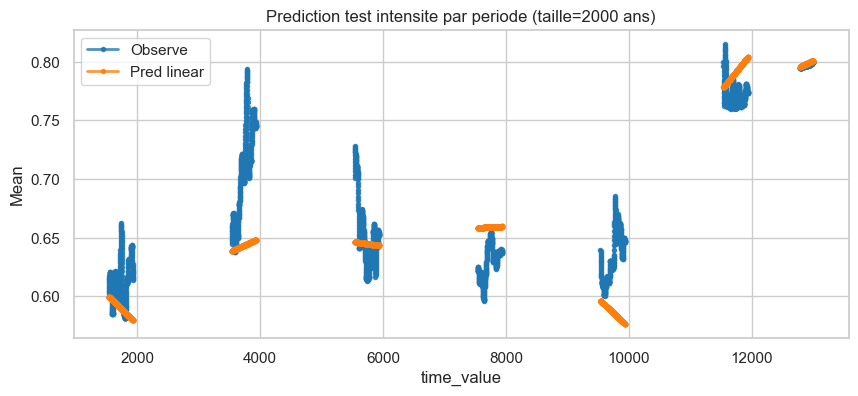
\includegraphics[width=0.92\textwidth]{figures_notebook_outputs/cell_009_output_18_09.png}
\caption{Prediction test pour une periode de 2000 ans.}
\end{figure}

\subsection{Conclusion sur la regression par periode}
La regression lineaire par periode capte correctement la tendance locale lorsque les fenetres sont courtes. En revanche, quand la periode augmente, la regression moyenne davantage les fluctuations et perd en precision sur les segments rapides de la serie. La lecture des figures suggere donc qu'un parametrage court est preferable si l'objectif est de suivre les ruptures et les transitions temporelles.

\section{Benchmark avec split aleatoire}

\subsection{Parametrage}
Le notebook compare plusieurs modeles sur un split aleatoire classique:
\begin{itemize}
\item proportion de test: 20\%;
\item graine de reproductibilite: 42;
\item modeles testes: DummyMean, Ridge, RandomForest et HistGradientBoosting;
\item preprocessing: imputation, standardisation des variables numeriques, encodage one-hot si necessaire.
\end{itemize}

Cette version est utile comme reference, mais elle doit etre interpretee avec prudence pour des series temporelles, car elle melange potentiellement des points proches dans le temps entre train et test.

\subsection{Resultats frequence}
Pour la frequence de feu regionale, les scores rapportes dans le notebook sont les suivants:

\begin{table}[H]
\centering
\begin{tabular}{lccc}
\toprule
\textbf{Modele} & \textbf{MAE} & \textbf{RMSE} & \textbf{$R^2$} \\
\midrule
RandomForest & 0.000003 & 0.000014 & 0.999893 \\
HistGradientBoosting & 0.000123 & 0.000152 & 0.987506 \\
Ridge & 0.000161 & 0.000203 & 0.977637 \\
DummyMean & 0.001110 & 0.001356 & -0.001198 \\
\bottomrule
\end{tabular}
\caption{Benchmark aleatoire sur la frequence de feu regionale.}
\end{table}

\subsection{Resultats intensite}
Pour l'intensite, le meme protocole donne:

\begin{table}[H]
\centering
\begin{tabular}{lccc}
\toprule
\textbf{Modele} & \textbf{MAE} & \textbf{RMSE} & \textbf{$R^2$} \\
\midrule
RandomForest & 0.000446 & 0.000748 & 0.999835 \\
HistGradientBoosting & 0.007744 & 0.011792 & 0.959018 \\
Ridge & 0.036026 & 0.044843 & 0.407376 \\
DummyMean & 0.046828 & 0.058251 & -0.000000 \\
\bottomrule
\end{tabular}
\caption{Benchmark aleatoire sur l'intensite.}
\end{table}

\subsection{Interpretation}
Le benchmark aleatoire montre que les modeles non lineaires dominent largement le baseline DummyMean. Toutefois, pour une serie temporelle, ces scores sont probablement optimistes car le split aleatoire permet de faire circuler de l'information temporellement voisine entre train et test. Pour une evaluation plus realiste, la regression par periode ou un split chronologique reste plus defendable.

\section{Synthese}
Les deux analyses ne racontent pas la meme histoire. La regression par periode met en evidence la structure temporelle locale et montre que le niveau de granularite temporelle change fortement la qualite du fit. Le split aleatoire, lui, donne de tres bons scores, mais il sert surtout de borne haute, pas d'estimation finale robuste.

\begin{itemize}
\item Si l'objectif est de lire la dynamique temporelle, il faut privilegier les fenetres courtes et la logique periodique.
\item Si l'objectif est de comparer des modeles rapidement, le split aleatoire fournit une reference utile mais optimiste.
\end{itemize}

\section{Sources}
Les figures et scores proviennent du notebook \texttt{exploration\_variables\_modeles\_feu.BACKUP.ipynb} et des images exportees dans \texttt{figures\_notebook\_outputs/}.

\end{document}